\section{Methodology}\label{sec: methodology}
Starting from a corpus of unstructured texts, we first use LLMs to extract the main characters from each document.
The characters are disambiguated and linked to a knowledge base if available.
We also create and store the document embeddings and character embeddings.
Then, we construct a document hypergraph and a character hypergraph, which are then clustered separately by combining connectivity similarity and semantic similarity.
The clustering result is hosted on the server and visualized in an interactive user interface.
Below, we describe each component in detail.
\subsection{Preprocessing}
The Methodology can work for any unstructured dataset
\subsubsection{Datasets}
% dataset references
~\cite{allthenews},~\cite{Isenberg:2017:VMC}, 
% OpenAI API website, used for embeddings and LLM
\footnote{\url{https://platform.openai.com}}

The scope of this research paper is to visualize diverse and unlabelled data conveying any type of information. Our testing is mainly focused on news articles and research papers to show results for all sorts of data. These news articles and abstracts are not domain specific and can be very abstract. \\
The following datasets were used:
\begin{itemize}
    % \item Roles Across Multiple Sentences (RAMS) - This dataset contains news articles with a wide variety of events. It contains 9,124 annotated events with 135 event types and 65 roles. We have used this dataset because of its abstract and wide ranging information that is not just restricted to a specific domain. 
    \item All The News - This dataset contains 143,000 articles from 15 American publications.  It typically includes metadata such as headlines, publication dates, and the full text of the articles. The dataset covers a wide range of topics, making it valuable for various natural language processing and text analysis tasks.
    \item Visualization Publications Dataset - This dataset contains information about IEEE visualization publications from 1990-2022. The purpose of using this dataset was to test our methods on majorly technical and scientific datasets. These research papers cover a wide-variety of research topics with fileds like abstracts, keywords, author names, titles ,number of citations, etc. The abstracts are used for the task of event extraction, where the event is the main research idea of the paper.This dataset is used to explore a new kind of event extraction where the definition of an event and main participants change in technical terms as compared to generic articles.
\end{itemize}
\subsubsection{Summarization}
Chatgpt for summarization
\subsubsection{Document Embedding}\label{sec: embeddings}
OpenAI's embedding API
\subsubsection{Character Extraction}\label{sec: character_extraction}
Chatgpt for major character extraction and another model for entity linking

\subsubsection{Topic Assignment}\label{sec: tag_assignment}
Chatgpt to assign topics to each cluster
~\cite{raval2023explainandtrust}
\subsection{Models}
\subsubsection{Hypergraph}
A hypergraph is a generalization of a graph in which an edge can connect any number of nodes~\cite{fischer2021hypergraphsurvey}.
A hyperedge thus represents a multi-way relationship between nodes.
In our work, we model two types of hypergraphs: document hypergraph and character hypergraph, where documents and characters are the nodes, respectively.
Analyzing the document hypergraph and character hypergraph correspond to topic-based and entity-based analysis, respectively.
Modeling the corpus as two hypergraphs allows us to support users to conduct both types of analysis simultaneously under a unified framework (\textbf{DC1}).

Following the definition of a hypergraph node, a hyperedge can be used to represent two types of multi-way relationships:
(1) A hyperedge between \textit{documents} can be constructed between documents that mention the same character. 
In this case, the hyperedge represents the co-mention of a character, i.e.\ a named entity or a concept;
(2) A hyperedge between \textit{characters} can be constructed between characters if they are mentioned together in the same document.
In this case, the hyperedge represents a co-occurrence relationship between characters.
Once the two hypergraphs are constructed, they are hierarchically clustered separately.
Clusters in the document hypergraph represent topics that are discussed in the dataset.
Clusters in the character hypergraph represent characters (entities or concepts) that frequently co-occurred in an article.
For better interpretability of the clustering result, we further assign \textit{tags} to each cluster, which is further explained in~\autoref{sec: tag_assignment}.

Although these two types of hyperedges are constructed differently, we utilize the \textit{dual} of a hypergraph to simplify the construction process.
The dual of a hypergraph is simply another hypergraph, where the hyperedges are now nodes and the nodes are now hyperedges, as shown in~\autoref{fig: duality}.
Therefore, we first model the documents as nodes and characters as hyperedges to construct the document hypergraph $H_A$.
The character hypergraph $H_P$ can then be easily constructed by taking the dual of $H_A$.
This construction process also allows us to use the same clustering algorithm on both hypergraphs, which is further explained in~\autoref{sec: clustering}.

\begin{figure}
 \centering % avoid the use of \begin{center}...\end{center} and use \centering instead (more compact)
 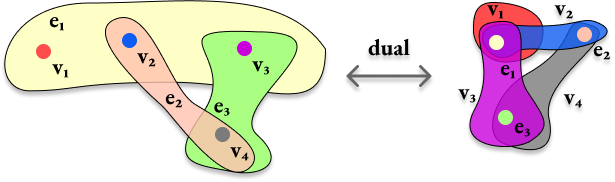
\includegraphics[width=\columnwidth]{duality}
 \caption{Illustration of the dual of a hypergraph. 
 Left: a hypergraph with 4 nodes $v_1, v_2, v_3, v_4$ and 3 hyperedges $e_1=(v_1, v_2, v_3), e_2=(v_2, v_3), e_3=(v_3, v_4)$. 
 Right: the dual of the hypergraph, where the nodes and hyperedges interchanged.
 Nodes in the dual hypergraph are now $e_1, e_2, e_3$ and hyperedges are $v_1=(e_1), v_2=(e_1, e_2), v_3=(e_1, e_3), v_4=(e_2, e_3)$.
 }
\label{fig: duality}
\end{figure}

\subsubsection{Hierarchical Clustering}\label{sec: clustering}
Common clustering algorithms for graphs consider only graph connectivity.
However, for the best interpretability of the clustering result, the node embeddings must be also used in the clustering process.
The necessity of incorporating node embeddings is further explained in~\autoref{sec: tag_assignment}.
Therefore, this limits our choice of clustering algorithms to attributed node clustering algorithms.

Although there are existing approaches that can cluster attributed nodes on graphs such as EVA~\cite{citraro2020eva} and iLouvain~\cite{combe2015louvain}, they are not designed for hypergraphs.
In general, hypergraphs can be clustered in two different ways: 
(1) Directly operate on the hyperedges by generalizing the graph clustering algorithms.
For example, Kamiński et al.~\cite{kaminski2021hgraphcommunity} generalizes the modularity metric for graphs to hypergraphs; 
(2) First transform the hypergraph into a graph and then apply normal graph clustering algorithms~\cite{kumar2020new}.
Although the first approach is more intuitive, it is less scalable and hard to incorporate node attributes.
Thus, we have decided to design our clustering algorithm following the second approach.

Considering all the above, we implemented our hierarchical clustering algorithm by first transforming the hypergraph into a graph following the edge re-weighting process proposed by Kumar et al.~\cite{kumar2020new},
then an agglomerative clustering algorithm~\cite{steinbach2000doccluster} is applied on the re-weighted graph.
In agglomerative clustering, the key is to define the similarity between nodes and similarity between clusters.
We can easily incorporate node attributes into the clustering process by defining the similarity between nodes and clusters as a combination of attribute similarity $S_s$ and connectivity similarity $S_c$.
Since we're dealing with texts, we refer to the attribute similarity between nodes as semantic similarity. 

The semantic similarity $S_s(i, j)$ is the cosine similarity of the embeddings of the two nodes, denoted as $v_i$.
For article nodes, the embeddings are generated using the article content.
For participant nodes, the embeddings are generated using a description note of the participant.
More details about the embeddings are explained in~\autoref{sec: embeddings}.
The connectivity similarity $S_c$ is the weighted Topological Overlap (wTO)~\cite{gysi2018wto},
which is a weighted generalization of the Overlap Coefficient~\cite{vijaymeena2016survey}, as shown in~\autoref{eq:connectivity_similarity}.
\begin{equation}\label{eq:connectivity_similarity}
    S_s(i, j) = \frac{v_i \cdot v_j}{||v_i|| \cdot ||v_j||}, \quad
    S_c(i, j) = \frac{\sum_{u=1}^N{w_{i,u}w_{u_j}} + w_{i,j}}{\min(k_i, k_j) + 1 - |w_{i,j}|}
\end{equation}
where $k_i = \sum_{j=1}^N |w_{i,j}|$ is the total weight of the edges connected to node $i$.
Finally, a weighting factor $\alpha$ is used to balance the two similarities, as shown in~\autoref{eq: similarity}.
\begin{equation}\label{eq: similarity}
    S = \alpha S_s + (1-\alpha) S_c
\end{equation}
For the similarity between clusters, we used centroid similarity, i.e.\ the similarity between two clusters is the similarity between the centroids of the two clusters.
The algorithm is presented in (TODO: add algorithm pseudocode here)


